% ============================================================================
% 5. EXPERIMENTS — Journal version (expanded with per-dataset tables)
% ============================================================================
\section{Experimental Results}
\label{sec:experiments}

\subsection{Evaluation Metrics}

We use \textbf{Exact Match (EM)} as the primary metric: a prediction is
correct if and only if it exactly matches the gold answer after
canonicalization (lowercase, sorted for unordered sets, shortest-path
tie validation against the FK adjacency matrix).
\textbf{F1 Score} provides token-level partial credit.

We report:
\begin{itemize}
  \item \textbf{Micro-EM}: Pooled exact match across all questions
    (total correct / total questions).
  \item \textbf{Macro-EM}: Mean of per-subtype exact match rates,
    weighting all 13~subtypes equally regardless of sample size.
\end{itemize}

\textbf{Target-node normalization.}
For \texttt{membership} questions of the form
``Which tables belong to the same connected component as table~$X$?'',
the queried table~$X$ is trivially always a member of its own component.
To avoid penalizing models for harmless self-inclusion or self-exclusion,
we strip~$X$ from both the prediction and gold answer before computing EM.
All \texttt{membership} scores in figures and tables use this normalization
unless explicitly noted as raw.  Raw EM averages 15\% for TU;
normalized EM averages 71\% (with Qwen reaching 100\%)---confirming
that the model correctly identifies all \emph{other} members but
inconsistently handles the self-reference of the queried node.

We include an \textbf{Oracle} baseline that injects gold graph algorithm
output into the prompt, establishing an upper bound.  All evaluations
use greedy decoding ($\tau{=}0$) for deterministic reproducibility.

\subsection{Tier~1: Main Results}

% TABLE 3: Main Results
\begin{table}[t]
\centering
\caption{Tier~1 schema-level results (Micro-EM~\% $\pm$ 95\% CI,
pooled across 5 datasets, 2000 bootstrap resamples).
\textbf{Bold}~=~best non-oracle.}
\label{tab:main-results}
\begin{tabular}{llccccc}
\toprule
Model & & FT & VR & GA & TU & RC \\
\midrule
Gemini & Micro & 76.6 & 72.9
  & 75.4 & \textbf{89.3}
  & 81.4 \\
\midrule
DeepSeek & Micro & 69.5 & 71.0
  & 76.8 & \textbf{90.4}
  & 79.4 \\
\midrule
Qwen & Micro & 63.2 & 69.5
  & 80.9 & \textbf{87.5}
  & 64.6 \\
\midrule
\multicolumn{2}{l}{\textit{Oracle}}
  & \multicolumn{5}{c}{99.5 / 99.8 / 100.0} \\
\bottomrule
\end{tabular}
\end{table}

\paragraph{Key Finding~1: Tool-Use dominates.}
Tool-Use achieves 89.3\% micro-EM (Gemini) and 90.4\% (DeepSeek),
outperforming the best static baseline by 13--14 percentage
points.

\paragraph{Key Finding~2: Static baselines show a Triviality Illusion.}
Flat Text appears competitive (76.6\% Gemini) because \texttt{join\_path}
(33\% of questions) inflates scores for baselines that handle FK
adjacency but fail on deeper tasks.

\subsection{Results by Difficulty}

% TABLE 4: By difficulty
\begin{table}[t]
\centering
\caption{Exact Match (\%) by difficulty level (pooled across 5 datasets).}
\label{tab:difficulty}
\begin{tabular}{llccccc}
\toprule
Model & Difficulty ($n$) & FT & VR & GA & TU & RC \\
\midrule
\multirow{3}{*}{Gemini}
  & Easy (544)   & 82.7 & 82.5 & 82.2 & \textbf{99.6} & 90.4 \\
  & Medium (300) & 78.9 & 73.0 & 76.3 & \textbf{90.3} & 78.7 \\
  & Hard (202)   & 56.1 & 46.5 & 55.6 & \textbf{59.9} & \textbf{60.9} \\
\midrule
\multirow{3}{*}{DeepSeek}
  & Easy (544)   & 82.7 & 84.4 & 87.1 & \textbf{98.0} & 88.8 \\
  & Medium (300) & 65.3 & 65.3 & 76.0 & \textbf{97.0} & 76.3 \\
  & Hard (202)   & 40.1 & 43.6 & 50.0 & \textbf{60.4} & 58.9 \\
\midrule
\multirow{3}{*}{Qwen}
  & Easy (544)   & 77.4 & 84.0 & 86.6 & \textbf{96.1} & 72.2 \\
  & Medium (300) & 57.7 & 63.0 & 90.7 & \textbf{92.0} & 64.7 \\
  & Hard (202)   & 33.2 & 40.1 & 51.0 & \textbf{57.4} & 44.1 \\
\midrule
\multicolumn{2}{l}{\textit{Oracle Hard}}
  & \multicolumn{5}{c}{99.0 / 99.5 / 100.0} \\
\bottomrule
\end{tabular}
\end{table}

\paragraph{Key Finding~3: Hard task plateau persists even with tools.}
Even Tool-Use plateaus on hard questions at $\sim$60\% EM versus Oracle's
$>$99\%.  Figure~\ref{fig:hop_decay} disaggregates EM by gold path length:
static baselines collapse beyond 3 hops (87\%$\to$19\% for FT), while
Tool-Use degrades more gracefully.

\begin{figure}[t]
\centering
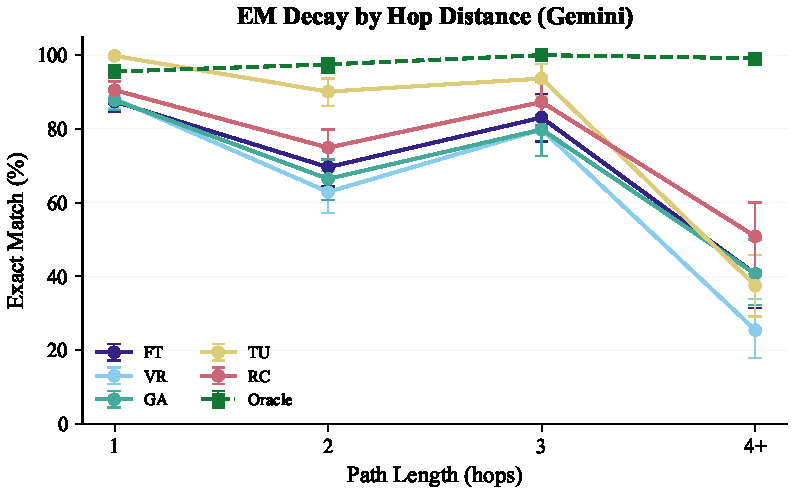
\includegraphics[width=0.9\linewidth]{figures/hop_distance_decay.pdf}
\caption{EM by gold path length.  Static baselines collapse
beyond 3~hops; Tool-Use degrades more gracefully but still falls short
of Oracle on long paths.}
\label{fig:hop_decay}
\end{figure}

\subsection{Per-Subtype Analysis}

\begin{figure}[t]
\centering
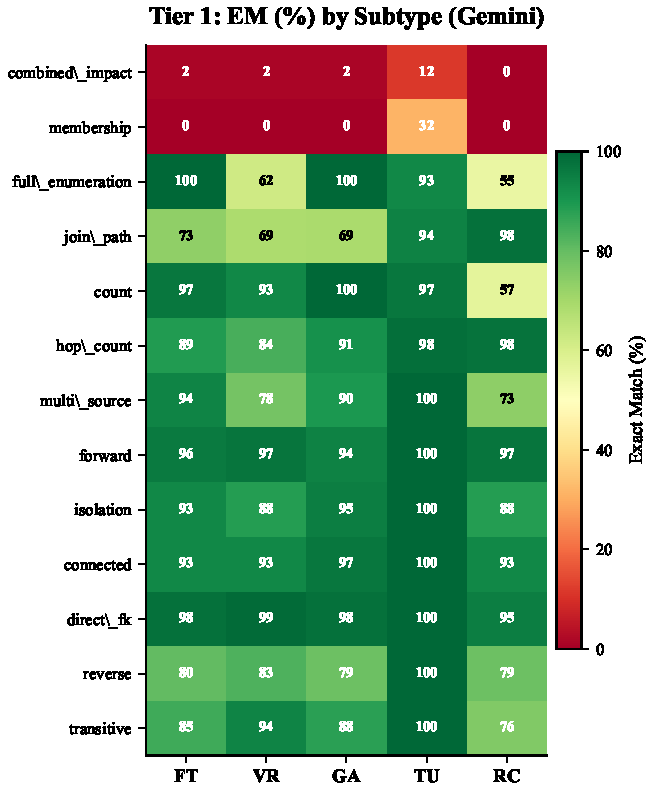
\includegraphics[width=0.95\linewidth]{figures/subtype_heatmap.pdf}
\caption{Tier~1 EM~(\%) by subtype for both models.
With target-node normalization, Tool-Use averages 71\% on
\texttt{membership} (with Qwen reaching 100\%), showing topology
enumeration is solvable with tools.
\texttt{combined\_impact} remains at 0--17\% across all baselines,
isolating compositional multi-hop reasoning as the core bottleneck.
\texttt{full\_enumeration} achieves 100\% for FT/GA because global
queries receive the full schema as context by design.}
\label{fig:heatmap}
\end{figure}

\paragraph{Key Finding~4: Retrieval-limited vs.\ reasoning-limited subtypes.}
Tool-Use achieves $\geq$93\% EM on subtypes requiring simple graph lookups
(\texttt{hop\_count}, \texttt{isolation}, \texttt{direct\_fk}).  However,
\texttt{combined\_impact} (12\% EM, $n=69$) remains intractable even with
tools.  For \texttt{membership}, raw TU EM is 15\%; after target-node
normalization (see Section~\ref{sec:experiments}), it rises to 71\%,
confirming that the bottleneck is self-reference inconsistency, not
an inability to enumerate component members.

\begin{figure}[t]
\centering

\includegraphics[width=\linewidth]{figures/difficulty_comparison.pdf}
\caption{Exact Match by difficulty.  All non-oracle baselines plateau
on hard questions.}
\label{fig:difficulty}
\end{figure}

\begin{figure}[t]
\centering
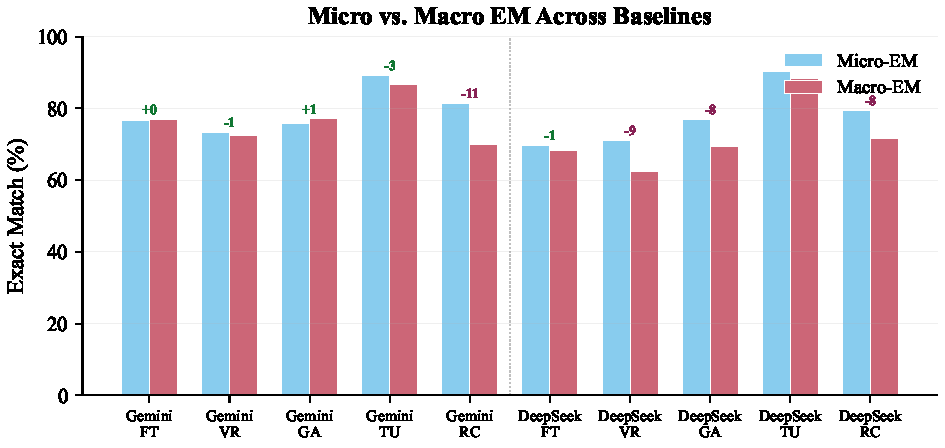
\includegraphics[width=0.9\linewidth]{figures/triviality_illusion.pdf}
\caption{Micro vs.\ Macro EM across baselines.  Negative deltas reveal
the Triviality Illusion effect.}
\label{fig:triviality}
\end{figure}

\subsection{Obfuscation Results}

% TABLE 5: Obfuscation
\begin{table}[t]
\centering
\caption{Obfuscation penalty: Micro-EM (\%) drop when table names are
replaced with random identifiers (4 datasets, excl.\ Syn-Logistics).}
\label{tab:obfuscation}
\begin{tabular}{llccccc}
\toprule
Model & & FT & VR & GA & TU & RC \\
\midrule
\multirow{3}{*}{Gemini}
  & Original    & 71.8 & 69.3 & 71.2 & \textbf{91.2} & 87.1 \\
  & Obfuscated  & 56.8 & 43.5 & 43.5 & \textbf{87.8} & 79.5 \\
  & $\Delta$    & $-$15.0 & $-$25.8 & $-$27.7 & $-$\textbf{3.4} & $-$7.6 \\
\midrule
\multirow{3}{*}{DeepSeek}
  & Original    & 68.4 & 74.5 & 82.3 & \textbf{91.4} & 83.4 \\
  & Obfuscated  & 40.5 & 42.6 & 57.7 & \textbf{87.2} & 84.0 \\
  & $\Delta$    & $-$27.9 & $-$31.9 & $-$24.6 & $-$\textbf{4.2} & $+$0.6 \\
\midrule
\multirow{3}{*}{Qwen}
  & Original    & 59.6 & 70.5 & 82.8 & \textbf{88.4} & 62.8 \\
  & Obfuscated  & 50.7 & 56.7 & 63.1 & \textbf{84.7} & 55.3 \\
  & $\Delta$    & $-$8.9 & $-$13.8 & $-$19.7 & $-$\textbf{3.7} & $-$7.5 \\
\bottomrule
\end{tabular}
\end{table}

\begin{figure}[t]
\centering

\includegraphics[width=0.9\linewidth]{figures/obfuscation_penalty.pdf}
\caption{Obfuscation penalty by baseline.}
\label{fig:obfuscation}
\end{figure}

Tool-Use shows minimal degradation ($\Delta{=}{-}3.4$\% Gemini,
${-}4.2$\% DeepSeek, ${-}3.7$\% Qwen) while static baselines lose 9--32
percentage points.  DeepSeek RC shows near-zero penalty
($\Delta{=}{+}0.6$\%), confirming that code execution against the graph
object is fully invariant to name perturbation.

\subsection{Tier~2: Value-Level Evaluation}

Tier~2 extends evaluation to value-level questions requiring interactive
data access.  The three remaining Tier~1 datasets (TPC-DS, TPC-DI, OMOP)
are schema-only releases containing no row-level data; value-level
evaluation is impossible on them by construction.  We evaluate Tier~2 on
\textbf{Syn-Logistics} (synthetic, 433~questions), the dataset with
fully materialized row-level lineage in this study, covering 8~subtypes
(Table~\ref{tab:tier2}).  AdventureWorks contains 520 Tier~2 questions in
the benchmark corpus but requires full ETL data hydration; evaluation is
ongoing work (see Limitations).

\begin{figure}[t]
\centering

\includegraphics[width=\linewidth]{figures/tier2_subtype.pdf}
\caption{Tier~2 value-level EM by subtype.
\texttt{cascade\_count} and \texttt{row\_provenance} require tools.}
\label{fig:tier2}
\end{figure}

% TABLE 7: Tier 2 (both models)
\begin{table}[t]
\centering
\caption{Tier~2 value-level results (EM~\%) on Syn-Logistics
($n{=}433$ questions across 8~subtypes).  Gemini and DeepSeek are
full evaluations; Qwen follows the same essential vs.\ insufficient
pattern and is fully detailed in Appendix~\ref{app:tier2}.}
\label{tab:tier2}
\small
\begin{tabular}{llcccccc}
\toprule
 & & \multicolumn{3}{c}{Gemini} & \multicolumn{3}{c}{DeepSeek} \\
\cmidrule(lr){3-5} \cmidrule(lr){6-8}
Subtype & $n$ & FT & GA & TU & FT & GA & TU \\
\midrule
cascade\_count      & 58  & 0   & 0   & \textbf{100} & 0   & 0   & \textbf{100} \\
row\_provenance     & 84  & 0   & 8   & \textbf{92}  & 0   & 7   & 11 \\
row\_impact         & 56  & 27  & 27  & \textbf{38}  & 25  & 25  & \textbf{59} \\
value\_origin       & 60  & 48  & 53  & 52           & 25  & 42  & \textbf{52} \\
multi\_hop\_trace   & 60  & 30  & 30  & 27           & 27  & 30  & 27 \\
value\_propagation  & 40  & \textbf{85} & 75  & 62   & \textbf{85} & 80  & 70 \\
cross\_silo\_reach. & 40  & 57  & 57  & 52           & \textbf{60} & 57  & \textbf{65} \\
shared\_source      & 35  & \textbf{37} & 26  & 23   & 26  & 20  & 20 \\
\midrule
\textbf{Overall}    & 433 & 30  & 31  & \textbf{59}  & 26  & 29  & \textbf{48} \\
\bottomrule
\end{tabular}
\end{table}

\paragraph{Key Finding~5: Tools are essential for value-level questions.}
\texttt{cascade\_count} achieves 100\% with tools versus 0\% without,
for \emph{both} models, confirming this is a structural necessity,
not a model-specific artifact.

\paragraph{Key Finding~6: Tools are necessary but insufficient.}
Despite solving data-access subtypes, Tool-Use achieves only 59\%
overall EM (Gemini) and 48\% (DeepSeek).  On \texttt{multi\_hop\_trace}
(27\% both models) and \texttt{shared\_source} (23\%/20\%), tools
provide no advantage.  DeepSeek's lower TU score (48\% vs.\ 59\%)
is driven primarily by \texttt{row\_provenance} (11\% vs.\ 92\%):
DeepSeek identifies the correct source \emph{tables} but returns
wrong \emph{row IDs}, indicating a failure in parsing tool output
rather than in tool selection, a model-specific instruction-following
gap on structured row-level results.

\begin{figure}[t]
\centering
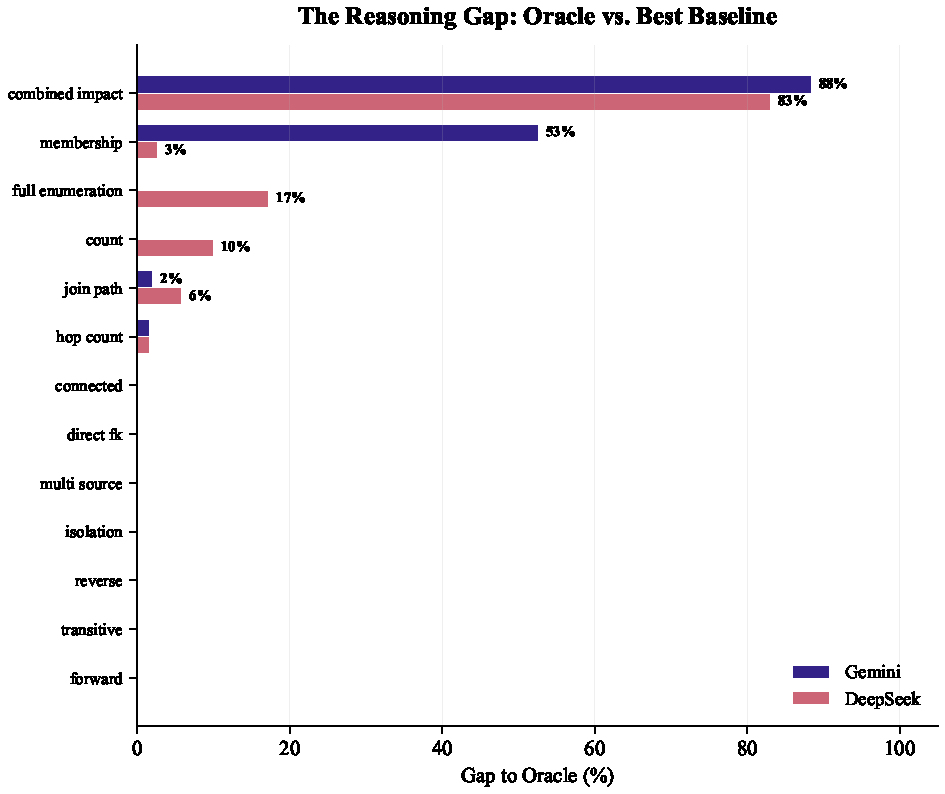
\includegraphics[width=\linewidth]{figures/oracle_gap.pdf}
\caption{The Reasoning Gap: Oracle~EM minus best non-oracle baseline
EM, per subtype. \texttt{combined\_impact} retains an 85+\% gap for
both models; 7 of 13 subtypes are effectively solved (gap~$<$~3\%).}
\label{fig:oracle-gap}
\end{figure}

\subsection{Limitations}

\textbf{Context Parity.} Baselines do not enforce strict token-budget
parity.  Since 45\% of questions involve paths exceeding 3 hops,
GA scores may be depressed on long-range subtypes.

\textbf{Baseline Coverage.} DeepSeek ReAct-Code is evaluated on all
5 datasets for original conditions and 4 datasets (excluding
Syn-Logistics) for obfuscated conditions.

\textbf{Statistical Treatment.} We use greedy decoding ($\tau{=}0$) with
a single deterministic pass for exact reproducibility.  Per-question
results are released for community bootstrap analyses.

\textbf{Model Breadth.} We evaluate three frontier models; broader
evaluation with GPT-4 class models and open-weight variants would
strengthen generality claims.  Tier~2 results for Qwen2.5-72B follow
the same tools-essential-yet-insufficient pattern (full results in
Appendix~\ref{app:tier2}); extending to AdventureWorks row-level
linkage is ongoing work.
